\chapterLabel{Results}

Running time for feature extraction + training + testing took on average 59
minutes on my i7, 3.4 GHz, 8 GB RAM machine. The above results were achieved
with pruning disabled, when enabled, accuracy went down and running time
increased.

\begin{figure}[H]
    \centering
    \caption{Results}
    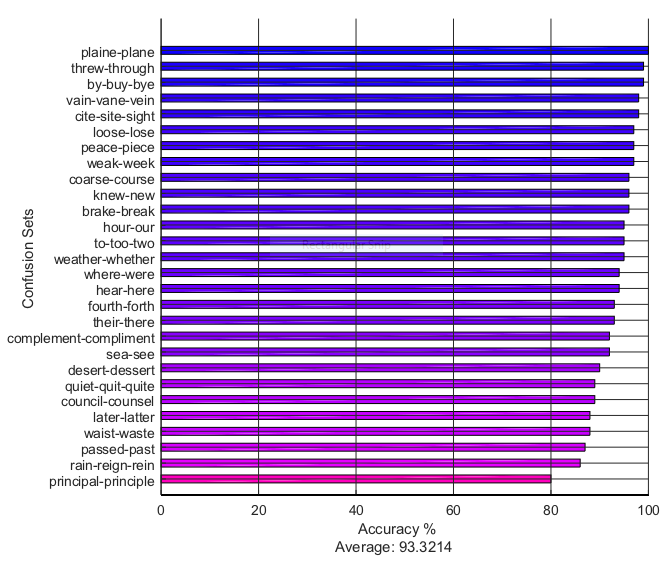
\includegraphics[width=135mm]{img/results.png}
\end{figure}

\sectionLabel{Key Features of Project}

\begin{enumerate}
\item Easily Extensible: New classification algorithms can be added easily as separate modules.
\item Very small footprint. Takes just 60MB of disk space and / or RAM.
\item Very fast algorithm. Can correct up to 20 sentences per second.
\end{enumerate}

\sectionLabel{Future Scope}

\begin{enumerate}
\item In training, for each word there's an array of classifiers, in the code I kept
the number to 1, we can add more algorithms like logistic regression or even
neural networks, then pick the best result using Weighted Majority Algorithm.
\item In context features extraction, we can use a dictionary API to properly stem
and singularize the tokens.
\item Soundex algorithm can be used to generate more confusion sets.
\item WordNET can be used to extract ‘concepts’ from the sentence and try to choose the correction candidate belonging to the same `concept'.
\item Multiple classifiers can be combined to provide better results and a more varied coverage of errors. e.g.\ TF-IDF, n-grams probability model etc.
\item A ranking algorithm can be used to give different weights to different classifiers.
\end{enumerate}
